\documentclass[11pt]{article}
\usepackage{geometry}                
\geometry{letterpaper}                   

\usepackage{graphicx}
\usepackage{amssymb}
\usepackage{epstopdf}
\usepackage{natbib}
\usepackage{amssymb, amsmath}
\usepackage{listings}
\usepackage{color}
\usepackage{a4page}
\DeclareGraphicsRule{.tif}{png}{.png}{`convert #1 `dirname #1`/`basename #1 .tif`.png}
\definecolor{listinggray}{gray}{0.9}

%\title{Title}
%\author{Name 1, Name 2}
%\date{date} 

\begin{document}



\thispagestyle{empty}

\begin{center}

\includegraphics[width=5cm]{ETHlogo.eps}

\bigskip


\bigskip


\bigskip


\LARGE{ 	Lecture with Computer Exercises:\\ }
\LARGE{ Modelling and Simulating Social Systems with MATLAB\\}

\bigskip

\bigskip

\small{Project Report}\\

\bigskip

\bigskip

\bigskip

\bigskip


\begin{tabular}{|c|}
\hline
\\
\textbf{\LARGE{Insert Title Here}}\\
\textbf{\LARGE{...}}\\
\\
\hline
\end{tabular}
\bigskip

\bigskip

\bigskip

\LARGE{Name 1 \& Name 2}



\bigskip

\bigskip

\bigskip

\bigskip

\bigskip

\bigskip

\bigskip

\bigskip

Zurich\\
May 2008\\

\end{center}



\newpage

%%%%%%%%%%%%%%%%%%%%%%%%%%%%%%%%%%%%%%%%%%%%%%%%%

\newpage
\section*{Agreement for free-download}
\bigskip


\bigskip


\large We hereby agree to make our source code for this project freely available for download from the web pages of the SOMS chair. Furthermore, we assure that all source code is written by ourselves and is not violating any copyright restrictions.

\begin{center}

\bigskip


\bigskip


%\begin{tabular}{@{}p{3.3cm}}
%\begin{minipage}{3cm}

%\end{minipage}
%&
\begin{minipage}{6cm}

\large Florian Besser

\end{minipage}
\bigskip \bigskip
\begin{minipage}{6cm}

\large Fabian M\"onkeberg

\end{minipage}
\bigskip
\begin{minipage}{6cm}

\large David Schwarz

\end{minipage}
%\end{tabular}

\end{center}
\newpage

%%%%%%%%%%%%%%%%%%%%%%%%%%%%%%%%%%%%%%%



% IMPORTANT
% you MUST include the ETH declaration of originality here; it is available for download on the course website or at http://www.ethz.ch/faculty/exams/plagiarism/index_EN; it can be printed as pdf and should be filled out in handwriting


%%%%%%%%%% Table of content %%%%%%%%%%%%%%%%%

\tableofcontents

\newpage

%%%%%%%%%%%%%%%%%%%%%%%%%%%%%%%%%%%%%%%



\section{Abstract}

This project presents an agent-based computational model of civil violence. Therein goes the central authority for it to suppress decentralized  rebellion. In general we build on an existing model of J.M.Epstein and try to make it more realistic by changing and adding certain properties of the ''agent'' and ''cop''. The focus of our work lies on the dynamics of the system and not on the political or social order. We are going to compare the results of our model, with those of J.M.Epstein.

\section{Individual contributions}

Abstract: Fabian and David\newline
Introduction and Motivations: Florian\newline
Description of the Model: David\newline
Implementation: Florian\newline
Simulation Results and Discussion: Fabian\newline
Summary: Fabian and David\newline
\newline\newline
Original Code: Florian\newline
Simulation run: David, with additional tweaks from Fabian\newline
\newpage

\section{Introduction and Motivations}

During the course of human history, regime changes have often occurred by civilians taking up arms. This “civil violence” also happens right now in Syria, and a similar movement has just been successful in Libya and Egypt. These uprisings or rebellions have a big impact on our world, and an ever bigger impact on the people actually executing them. So it is imperative to be able to predict such changes, and that's exactly what we strife for: A clear model for civil violence,so that in the future we can better predict outcomes and aftermaths of these events.\newline\newline
Real world examples: Syria, Libya, Egypt, Russia, United States of America, even Switzerland etc.\newline
(The canton Wallis had various unsuccessful uprisings until it was granted autonomy from Bern.)\newline\newline
Today, as taught in our schools, revolutions are formed by “normal”civilians, who are unhappy with their current situation. Somehow, this unhappy (but non-active) mob produces/elects a leader, who will then lead them into action. This now active mob will then have to fulfill certain tasks, such as taking up weapons against an oppressive military force, or a demonstration of force in form of a peaceful protest. On completion of these tasks, they can then form their own government according to their liking.\newline
While the very first step (unhappy civilians) is often a requirement, the idea of a revolution forming and a revolution marching against the current system is not sophisticated enough. There are many factors which can catalyze or hinder the formation of a rebellion, as we are going to show.\newline\newline
The tactics which can be employed by a system that is under attack are also somewhat left out in our education, take the revolution in Egypt as an example: What would have happened if the government went “all out” on the protesters? Would the military rule have held another decade?

\newpage

\section{Description of the Model (Cop/Agent)}

This is an agent-based model about civil violence. We look at a model were the central authority goes for it to suppress decentralized rebellion. We don't take respect to political or social order, it is just a general case. It is based on the model of J.M.Epstein.
This model differs between two main actors. ''Agents'' are members of the general population and may be actively rebellious or not. ''Cops'' are the token of the central authority, which arrest actively rebellious agents. Later we will make some more sophisticated characterizations, trying to do a more precise and realistic simulation. J.M.Epstein tried to get recognizable macroscopic revolutionary dynamics of fundamental interest with a model, that is as idealized as possible. We try to improve this model. It is now interesting, if we can make remarkable refinements, such that this model is more realistic. 
First I will describe the agents.
The original part is always from the idea of J.M.Epstein and then the additional specifications are our own ideas and extensions.

\subsection{The original agent specification}
To simulate a rebellion each agent needs some properties, on which we can measure the feelings of them. Therefore there must be some representation of political grievance. The treatment of this model will be really simple and is denoted by two idealized components, which are called hardship (\textbf{H}) and legitimacy (\textbf{L}). Their definitions are as follows:\\
\textbf{H} is the agent's perceived hardship (i.e., physical or economic privation). It is defined exogenous and it is assumed to be heterogeneous across agents. It is simply presumed to be uniformly distributed on the interval (0,1). An other important factor is \textbf{L}, the perceived legitimacy of the regime. This is exogenous and is equal across agents. In the different runs, it will be varied over the interval (0,1).\\
This two properties can be combined to the level of grievance any agent feels towards the regime. It is suggested, because of the many functional relationships as: 
\begin{equation}
G=H(1-L)
\end{equation}
Grievance is the product of perceived hardship (\textbf{H}) and perceived ''illegitimacy'' (\textbf{1-L}). The intuition behind this formula is simple. If you think it is legitimate how the government acts (high \textbf{L}) then you will not revolt, do not matter how bad things are going on. And if the perceived hardship is pretend to be low, then the grievance towards the regime will be low, too. It does not matter what the perceived illegitimacy is.
Because the decision to rebel depends on more than one's grievance, there is defined \textbf{R} as the agent's level of risk aversion. Heterogeneous across agents, this is assumed to be uniformly distributed on (0,1) and it is fixed for the agent's lifetime.\\
Everyone thinks before getting active, what the current risk is to get arrested and this is assumed to be proportional with the cop-to-active ratio (\textbf{C/A}){\footnotesize v} within vision \textbf{v}. Where the vision \textbf{v} is defined as the agent's vision, this is the number of lattice positions (north, south, east and west of the agent's current position) that the agent is able to inspect. Now is the agent's estimated arrest probability \textbf{P} defined by
\begin{equation}
P=1-exp[-k(C/A){\footnotesize v}]
\end{equation}
The constant $k$ is set to ensure a plausible estimate (of \textbf{P} = 0.9) when \textbf{C}=1 and \textbf{A} = 1. Notice that (\textbf{C/A}){\footnotesize v} is always defined, because the agent counts always with himself as active, so  \textbf{A} is at least 1.
Finally we define the agent's net risk \textbf{N} = \textbf{RP}, what is the product of his risk aversion and estimated arrest probability. This is the special case of \textbf{N} = \textbf{RPJ\textsuperscript{$\alpha$}}, where \textbf{J} is the jail term, as discussed in Epstein.
A quiescent agent is called an agent in state Q and an active agent is called an agent in state A. Now we can write down the agent's rule:
\begin{equation}
Agent~ rule ~A: If~ G - N > T ~ be~ active; otherwise, be~ quiet.
\end{equation}
Typically , T is set at some small positive value.
So we consider, that the agents weigh expected costs and benefits rationally.

\subsection{Additional agent specification}
Our aim was now, to get a better simulation for revolutions. In the real world, there is a point on which the people try to kill the cops and vice versa. Therefore we implemented a murder threshold \textbf{T\_murder} and if (\textbf{G} - \textbf{N}) $>$ \textbf{T\_murder}, then he tries to kill cops. Therefore exists a \textbf{murder success rate} and a \textbf{murder assassin death rate}, which define his success by murdering cops and the probability, that he dies during this action, himself. This means, that if a certain level is reached, the agents can now murder cops, too.  \\
During an arrest, there can occur some trouble. Therefor, there exists the \textbf{agent death chance}, the probability, that the agent dies during this conflict. And the \textbf{cop death chance} is the probability, that the cop dies.
If we have the first case, that an agent dies, then the legitimacy drops by the \textbf{agent death legitimacy penalty}. And if a cop dies, then the legitimacy increases by the \textbf{cop death legitimacy boost}.\\ 
With this new attribute, we hope to get a new dynamic. Because if cops are murdered, then the (\textbf{C/A}){\footnotesize v} will drop and so there can go more agents active. Otherwise if a agent dies, there is the \textbf{agent death legitimacy penalty} for balancing the raised  (\textbf{C/A}){\footnotesize v}. \\
Again a unreal setting of the original version is that everyone has the same legitimacy. For that we define the \textbf{legitimacy\_mod}, so that the personal legitimacy equals $L + L\_personal$, where L\_personal is a value out of U(-legitimacy\_mod,legitimacy\_mod). This means, that we have a certain variance of personal legitimacy.
Now we may have agents with an higher personal legitimacy and go earlier active than the others. This means,that they are a trigger for other agents to go active and so we have a starting point of a revolution.

\subsection{The original cop specification}
The cops are much simpler than the agents. The properties of them are:\\
\textbf{v\textsuperscript{$\ast$}} is the cops vision and it is like \textbf{v} the number of lattice positions that the cop is able to inspect. It is exogenous and equal across cops. But it does not have to be equal to \textbf{v}.
The rule, with which the cops operate is:
\begin{equation}
Cop~rule~C:~Inspect~all~ sites~ within~v\textsuperscript{$\ast$}~and~arrest~a random~active~agent.
\end{equation}
In the basic model of J.M.Epstein cops never defect to the revolution.

\subsection{Additional cop specification}
Because cops are human, too, the government can not do whatever they want to do with them. After a certain point (see rule S), they realize, that they do not want to work for the government anymore and stop their work. If it gets even worse, then they can defect (go to the agents).\\
Then we thought about this, how to model. And we have got the result, that we have to introduce a legitimacy for the cops, too. Therefore they get the same basic legitimacy like the agents, but with an other interval for the personal legitimacy change. And then the personal legitimacy equals  $L + L\_personal$, where L\_personal is now a value out of U(-legitimacy\_mod\_cop,legitimacy\_mod\_cop).\\
Therefor we define two new rules:
\begin{align*}
Stop~rule~S:~If~L+L\_personal \leq legitimacy\_threshold\_stop ,\\
then~he~will~not~arrest~agents~anymore.
\end{align*}

\begin{align*}
Defect~rule~D:~If~L + L\_personal \leq legitimacy\_threshold\_defect,\\
then~the~ cop~transforms~to~an~agent.
\end{align*}

It is clear, that legitimacy\_threshold\_defect $\leq$  legitimacy\_threshold\_stop. 


\subsection{Movement and Jail Terms}
One fundamental property of people, is the movement. This gives the whole model a certain dynamic, because the agent information (the number of cops and actives they see) is heterogeneous. And this dynamic will change, by changing \textbf{v} and \textbf{v\textsuperscript{$\ast$}}. The movement rule is the same for both agents and cops:
\begin{equation}
Movement~rule~M:~Move~to~a~random~site~within~your~vision.
\end{equation}

For the jail term, the user set a a value for the maximum jail term, \textbf{J\_max}. Then, any arrested active is assigned a jail term drawn randomly from U(0,\textbf{J\_max}). This is an important term in the model, which handles the duration of removing actives from circulation. If you set alpha to zero, there will be no deterrent effect of increasing the jail term.

\subsection{General changes of the model}
To anlyse some scenarios we implemented  the \textbf{each\_round\_legitimacy\_change}. If you set it not equal to zero, the legitimacy (\textbf{L}) will change every round by this factor. And so you can see what happens if the legitimacy of the government drops constantly.
To get even more heterogeneous agents and cops, we let the vision\textbf{v} and \textbf{v\textsuperscript{$\ast$}}, of the agents and cops, be various and uniformly distributed in (vision\_Min\_agent,vision\_Max\_agent) and in (vision\_Min\_cops,vision\_Max\_cops).\\
One last diversification is, that in the beginning all the cops start in the middle of the space and than move from there on. This should be the scenario, that the agent can communicate, where they will meet and the cops get the information not until they met!

\newpage

\section{Implementation}

The implementation of our model brings many features, as well as some added complexity.\newline
A short overview about the core functionality:\newline

\subsection{Problem Generation}
According to user-set constants, the playfield is filled with Agents and Cops. These players are generated with alle the required functionality to later perform their actions. Agents, for example, are already equipped with Hardship.
\subsection{Step}
Since the problem is now specified, we can loop one step at a time, until we reach some final state. In each step, there are a few things that must be done:
\subsubsection{Reset Moves}
Every Cop and Agent can move exactly once per step, so we must ensure that they can now move properly.
\subsubsection{Release imprisoned}
All the imprisoned Agents have their sentence reduced by one. All Agents with a sentence of zero or less are set free. They are randomly put onto empty fields on the playfield.
\subsubsection{Move Cops and Agents}
Agents scout out the empty fields in their vision, and choose one at random. In case there are no empty fields, they stay put.\newline
Cops scout for active Agents, as well as empty fields. If they spot an Agent, they move to the Agent's field and arrest him. Should no Agent be inside the Cop's vision, they randomly move to an empty field. In case they can'tfind an Agent or an empty field, they stay put.
\subsubsection{Set Status of Agents}
With all the Agents and Cops moved, the Agents need to re-evaluate whether they want to be active. Their activeness is set for the next round, as well as for display purposes. Cops as well as empty squares are also saved for display.
\subsubsection{Display current Model}
With the saved values from the step above, a graph can be plotted, showing all Agents and Cops, as well as some info about them.
\subsection{Display summarizing plots}
At the very end, plot some graphs of the most important values during the computation. Current graphs include active Agents, inactive Agents, imprisoned Agents, active Cops, Legitimacy.

\subsection{Tweaks}
This core model has been enhanced by many tweaks and options, listed here:
\subsubsection{Size}
The size of the playfield can now be changed.

\subsubsection{Occupied to Unoccupied Ratio}
This ratio regulates Occupied Spaces vs. Unoccupied Spaces. In the original paper, the author started with a full playfield, but that might not always be desired.

\subsubsection{Cop to Agent Ratio}
This ratio sets the global amount of Cops vs. Agents. Especially useful when simulating low/heavy police presence with varying playfield size.

\subsubsection{Jailterm Min/Max}    
Minimum and Maximum amout of steps an Agent will spend in jail if arrested.

\subsubsection{Jail sentence}
In the original paper, the jail sentence was chosen uniformly from zero to some maximum. In reality, jail sentences are not chosen uniformly, and so this function can be altered in whatever way desired. It uses the Jailterm Min/Max discussed above.

\subsubsection{Jail Aggreviance}
In the original paper, released Agents left the jail just as aggrieved as when they were captured. Modeling different criminal justice systems is nearly impossible that way.Therefor, we implemented this variable. If Agents are badly treated in jail, they now will be released in an angry state.

\subsubsection{Activism Threshold}
The attitude of an agent against the regime is computed by subtracting the net risk of arrest for that agent from his personal grievance. But what attitude is needed for an Agent to actually go active? In the original paper, this was assumed to be zero, but we implemented a variable to model different people and their resistance to regimes.

\subsubsection{Murder Threshold}
In order to model militant uprisings we needed some functionality for Agents to actually kill or at least attack Cops. This murder threshold is the outcome. Normally much higher than the activism threshold, if fulfilled, the Agent will no longer protest but instead go and hunt down Cops.

\subsubsection{Murder success rate}
Depending on the tools available to murdering Agents, they may or may not succeed in killing a cop. This is used to differentiate between countries with easy/difficult access to weapons for civilians.

\subsubsection{Murder assassin death rate}
Sometimes Agents might get killed while trying to kill a Cop. If the Cops are taken by suprise the revolution might go much more smoothly than if all Cops are heavily armed and have orders to kill every attacker.

\subsubsection{Vision Min/Max}
These variables, separate for Agents and Cops, govern the visible field. In every step, players can only gauge what happens in their fieldof vision, and act upon it. Large fields of vision will allow Cops to become more effective, while Agents can better interpret their chances of getting arrested.

\subsubsection{Death}
Whenever a Cop tries to arrest an Agent, either one of them might die. As seen in 2008 in Greece, the death of Alexandros Grigoropoulos sparked violence. So whenever an Agent dies while being arrested, the Legitimacy of the regime suffers. To somewhat even out the effect, in case a Cop dies, the Legitimacy receives a boost. These variables are especially useful when gauging if a regime should use many Cops to quickly crack down on Agents, or whether they should use a moderate force to slowly curb the unrest.

\subsubsection{Important Places}
In the original paper, Cops as well as Agents wander pretty much randomly. When modeling Egypt's revolution in and around Tahir square, the idea of randomly moving doesn't cut it. Both Agents and Cops marched to one important place, and then clashed there. To model such an important point, this feature was added.

\subsubsection{Important people}
Nerly every revolution had it's heroes. While they were not so powerful by themselves, they would often tip the balance in their favor. We modeled important people with an extended Vision, as well as enhanced effectiveness: When an Agent tries to find out his chances of arrest, he will measure a low chance when standing next to an important Agent, but a very high chance when seeing an important Cop.

\subsubsection{Defective Cops}
Normally, Cops won't defect to the Agents side. In special cases, such as Egypt and Tunesia, the Cops decided to join the Agents since the Legitimacy of the regime had fallen too low. We modeled this using two variables. Should the Legitimacy fall below some threshold, Cops will stop arresting Agents. If the Legitimacy falls further, they will abandon their post and join the Agents.

\subsubsection{Better Legitimacy}
Legitimacy is normally not globally percieved. Some people will always agree with a certain regime, while others will always disagree. To model such cases, we assigned every Agent and Cop his own impression of the regime. This allows for some more believable outcomes, such as Agents with low Hardship but a distinct hatred of the regime going active, as well as Agents with high Hardship keeping silent because they love the regime.

\subsubsection{Legitimacy Change each step}
In certain cases a regime might loose supporters as time passes. For example the people of Egypt are pressing for reforms, and the longer they have to wait, the less satisfied they will become with the regime. This variable can be used to model such cases, and help decide when the breaking point is reached, by which a reform needs to be introduced, or the protests will start again.

\subsubsection{Number of Frames}
This variable does not have any influence on the computation itself,but governs how many steps are computed and archived.

\subsubsection{Plot every X Frames}
In case the number of frames ishigher than five, one might want to consider notplotting each and every step, and this variable governs that.

\newpage

\section{Simulation Results and Discussion}

%USE THE FUNDAMENTAL QUESTIONS POSED IN THE PROPOSAL

\subsection{Comparison of Epstein Model with our Model}

\includegraphics{Picture1.png}

As in the Epstein model it can happen that the local cop to agent ratio drops too low and agents turn active. Later when the cops return the active agents disappear again either by arresting or turning inactive.  A good example for that is round 250. Since there are no cops in one corner agents turn active. The simulation was done with the following input: \newline
L = 0.7;\newline
O\_to\_U\_Ratio = 0.5;     \newline
C\_to\_A\_Ratio = 0.1;      \newline
Jailterm\_Min = 3;          \newline
Jailterm\_Max = 5;          \newline
Activism\_Threshold = 0.1;\newline
Vision\_Min\_Cops = 5;\newline
Vision\_Max\_Cops =7;\newline
Vision\_Min\_Agent = 5;\newline
Vision\_Max\_Agent = 7;\newline

All the other variables have been set to 0.\newline

\includegraphics{Picture2.png}\newline
\includegraphics{Picture3.png}\newline
\includegraphics{Picture4.png}\newline
\includegraphics{Picture5.png}\newpage

In the next graph we plot the number of active agents in every round. There is a sudden drop in the first couple of rounds: In the first round there are 116 active agents. But later the number of active agents is never larger than 60. Also can be observed that the number of active agents and the number of imprisoned agents affect each other. If the number of active agents is high the number of prisoner will probably be low and if only a few agents are active the prisoner will probably be full and vice versa.\newline

\includegraphics{Picture6.png}\newline
\includegraphics{Picture7.png}

\subsubsection{Salami Tactics of Corruption}
As in the Epstein model we studied the influence of a Change in legitimacy. We looked at two cases: A sudden drop in legitimacy and a smoothly decay in legitimacy. Booth cases happened in the real world. A very good example for a sudden legitimacy drop is Greece. After a protester was shot during a demonstration the public opinion suddenly dropped and the demonstration became even bigger.  An example of a smoothly decay is Egypt. The system seemed to by quiet stable but the lack of a better future for a whole generation steadily decreased the legitimacy.\newline

\subsubsection{Sudden drop}
We started with a legitimacy of 0.9.  Than in round 10 we reduced the legitimacy by -0.3.  This leads to a sudden increase of the number of active agents. Since the central force is very strong (number of Cop/agents =0.2) the number of active agents declines again and the prison gets full.

\includegraphics{Picture8.png}

L=0.9\newline
O\_to\_U\_ratio=0.5\newline
C\_to\_A\_Ratio=0.2\newline
Jailterm =(8,25)\newline
Activism\_Treshold=0.1\newline
Vision=7

\subsubsection{Linear decrease}
In this case all the parameters are exactly the same as above. The only difference is the Legitimacy. Instead of a sudden drop we reduced the legitimacy round by -0.6/200. In this case we don’t observe a peak in the number of active agents. Since the central force is strong and the prison terms rather long the cops can handle the situation.

\includegraphics{Picture9.png}

L=0.9\newline
O\_to\_U\_ratio=0.5\newline
C\_to\_A\_Ratio=0.2\newline
Jailterm = (8, 25)\newline
Activism\_Treshold=0.1\newline
Vision=7

\subsection{Influence of Cop Distribution}
We wondered what would change if we would let star the cop in the middle instead of randomly distributed and how does the influence of the starting position of the cops depends on their view.\newline
The idea is the following: In the beginning 49 cops are stationed in the middle of the field. Then they spread out and suppress the demonstrations. The question is now: How many rounds does it takes until the cops starting in the middle are as successful as the ones starting randomly.\newline
The following plot shows the field in the first round and in the 100 round. \newline\newline
Centre\newline\newline
\includegraphics{Picture10.png}\newpage
Random\newline\newline
\includegraphics{Picture11.png}\newline

Centre\newline\newline
\includegraphics{Picture12.png}\newpage
Random\newline\newline
\includegraphics{Picture13.png}\newline


There's clearly a big difference in the first round, but after 100 rounds the plots looks alike. \newline
We run the simulation with the following parameters: \newline
L=0.8\newline
O\_to\_U\_Ratio =0.7\newline
Jail = (3,6)\newline
Activism\_threshold=0.1\newline
Vision = (1,3)\newline
In the case of randomly distributed cops we set the C\_to\_A\_Ratio to 0.0743. So expected value of cops is 49 as in the case of cops starting in the centre.\newline\newline

In the following two graphs we clearly see that the cops starting in the middle are less successful in suppressing active agents and filling up the prison.\newline\newpage

Centre\newline
\includegraphics{Picture14.png}\newline
Random\newline
\includegraphics{Picture15.png}\newline

To get a more accurate result we took the mean and standard deviation of the number of active agents and the number of active agents over 30 runs of the simulations. We did that for 3 different tips of view ranges:\newline\newline

\subsubsection{View randomly distributed in (1,3)}

\includegraphics{Picture16.png}

After 60 rounds the cops starting in the middle are still clearly less successful in suppressing active agents than randomly distributed cops. Also the shapes of the curves doesn’t look alike\newline\newline

\includegraphics{Picture17.png}

The cops on the middle need 60 rounds until they finally have imprisoned as many agents as the randomly distributed cops.\newline\newline

\subsubsection{View randomly distributed in  (3-5)}

\includegraphics{Picture18.png}

In this case it takes the cops starting in the middle about 25 rounds to get as successful in suppressing the active agents as the randomly distributed cops. \newline\newline

\includegraphics{Picture19.png}

The curve in the random case after round 5 looks like the curve in the centre case after round 30. This holds also for the graph of active agents.\newline\newline

\subsubsection{View randomly distributed in  (5-7)}

\includegraphics{Picture20.png}

In this case the curves in the centre case shifted by about 5 rounds to the right looks like the curves in the random case. If we would increase the view even more the difference between the two cases would disappear completely. This is clear since we have only a 40* 40 field. So after about 4 moves of length 10 a cop starting in the middle can reach every position in the field.\newline\newline

It is also very interesting how the whole system behaves: After a number of rounds depending on view, population density and cop density  the average of the simulations gets constant.  \newline\newline

\subsection{Problems}

\subsubsection{View}
We get a problem with our simulation if the view is very low and in the same time the population density is high. An Example for that are the plots of the field in the chapter Influence of Cop Distribution.\newline
There we have a view in (1,3) and a ratio of 0.7 of occupied to unoccupied fields. After 100 rounds the people aren’t randomly distributed anymore. They sort of glue together in the corner. Since the view is small most of the people in this accumulation can’t move at all.\newline\newline

\subsubsection{Movement}
Our agents and cops can only move left, right, up and down. This seems to be not very realistic. If only one cop is in a particular region the situation can be very unrealistic. But if many agents are in a particular area they can cover the whole area with their movement and the situation is similar to the case there the cops can move in all directions. So always place enough cops in the field. The same also holds for agents. Enough means at least more than 40.

\newpage

\section{Summary and Outlook}

Summary and Outlook\newline
We implemented the basic idea of the Epstein and added several extra variables to simulate things as active agents trying to kill a cop, agent killed while trying to kill a cop, a cop or an agent killed during imprisonment, legitimacy influenced by a deadly incident during imprisonment, a personal legitimacy for every agent and cop, cops being more human i.e. stop working or even defect if legitimacy is too low.\newline
We compared our (basic) model in some simple cases with the Epstein model and got similar results. WE also studied the limitations of our model. We had a closer look on the influence of the starting position of the cops depending on their view.  Very interesting was the fact that in a couple of cases the mean over several simulations became constant after a couple of rounds. It would be interesting to check if this happens always or if their exist cases there the average doesn’t get constant but maybe behave periodic.

\newpage

\section{References}

Modeling civil violence: An agent-based computational approach, Eppstein 2002

\section{Appendix A: Proposal}

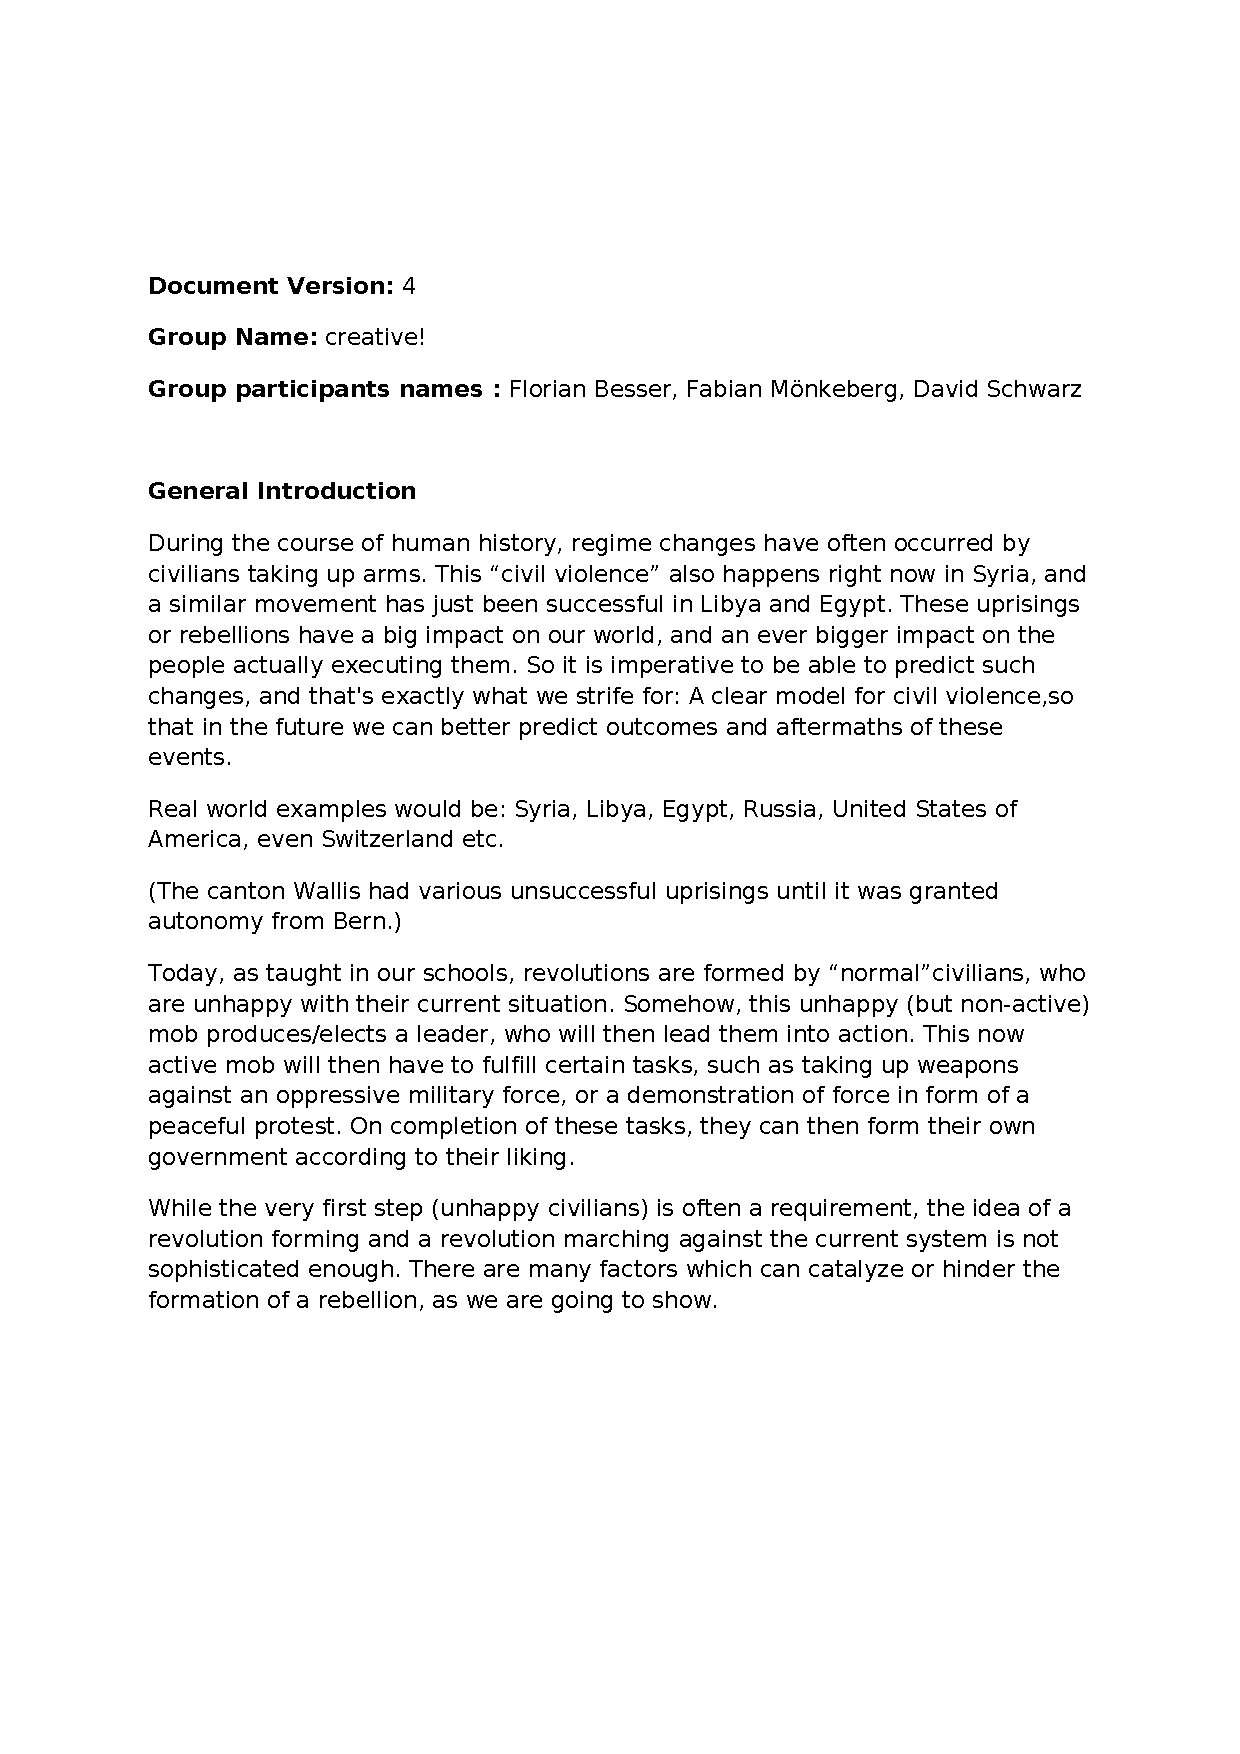
\includegraphics[bb=1.0in 1.0in 7.5in 10in,page=1]{Proposal.pdf}
\newpage
\includegraphics[bb=1.0in 1.0in 7.5in 10in,page=2]{Proposal.pdf}
\newpage
\includegraphics[bb=1.0in 1.0in 7.5in 10in,page=3]{Proposal.pdf}

\section{Appendix B: Code}

Listing from source file \texttt{Agent.m} \\

%---------------------------------------------------------------
\lstset{language=matlab}
\lstset{backgroundcolor=\color{listinggray},rulecolor=\color{blue}}
\lstset{linewidth=\textwidth}
\lstset{commentstyle=\textit, stringstyle=\upshape,showspaces=false}
\lstset{frame=trBL,frameround=tttt}
\lstinputlisting[caption=Agent,label=lst:Agent]{Agent.m}
%---------------------------------------------------------------

Listing from source file \texttt{Cop.m} \\

%---------------------------------------------------------------
\lstset{language=matlab}
\lstset{backgroundcolor=\color{listinggray},rulecolor=\color{blue}}
\lstset{linewidth=\textwidth}
\lstset{commentstyle=\textit, stringstyle=\upshape,showspaces=false}
\lstset{frame=trBL,frameround=tttt}
\lstinputlisting[caption=Cop,label=lst:Agent]{Cop.m}
%---------------------------------------------------------------

Listing from source file \texttt{Display.m} \\

%---------------------------------------------------------------
\lstset{language=matlab}
\lstset{backgroundcolor=\color{listinggray},rulecolor=\color{blue}}
\lstset{linewidth=\textwidth}
\lstset{commentstyle=\textit, stringstyle=\upshape,showspaces=false}
\lstset{frame=trBL,frameround=tttt}
\lstinputlisting[caption=Display,label=lst:Display]{Display.m}
%---------------------------------------------------------------

Listing from source file \texttt{Displaycentre.m}, changes only \\

%---------------------------------------------------------------
\lstset{language=matlab}
\lstset{backgroundcolor=\color{listinggray},rulecolor=\color{blue}}
\lstset{linewidth=\textwidth}
\lstset{commentstyle=\textit, stringstyle=\upshape,showspaces=false}
\lstset{frame=trBL,frameround=tttt}
\lstinputlisting[caption=Display,label=lst:Display]{Displaycentre.m}
%---------------------------------------------------------------

Listing from source file \texttt{Displayline.m}, changes only \\

%---------------------------------------------------------------
\lstset{language=matlab}
\lstset{backgroundcolor=\color{listinggray},rulecolor=\color{blue}}
\lstset{linewidth=\textwidth}
\lstset{commentstyle=\textit, stringstyle=\upshape,showspaces=false}
\lstset{frame=trBL,frameround=tttt}
\lstinputlisting[caption=Display,label=lst:Display]{Displayline.m}
%---------------------------------------------------------------

Listing from source file \texttt{Empty.m} \\

%---------------------------------------------------------------
\lstset{language=matlab}
\lstset{backgroundcolor=\color{listinggray},rulecolor=\color{blue}}
\lstset{linewidth=\textwidth}
\lstset{commentstyle=\textit, stringstyle=\upshape,showspaces=false}
\lstset{frame=trBL,frameround=tttt}
\lstinputlisting[caption=Empty,label=lst:Empty]{Empty.m}
%---------------------------------------------------------------

Listing from source file \texttt{Field.m} \\

%---------------------------------------------------------------
\lstset{language=matlab}
\lstset{backgroundcolor=\color{listinggray},rulecolor=\color{blue}}
\lstset{linewidth=\textwidth}
\lstset{commentstyle=\textit, stringstyle=\upshape,showspaces=false}
\lstset{frame=trBL,frameround=tttt}
\lstinputlisting[caption=Field,label=lst:Field]{Field.m}
%---------------------------------------------------------------

Listing from source file \texttt{select_field.m} \\

%---------------------------------------------------------------
\lstset{language=matlab}
\lstset{backgroundcolor=\color{listinggray},rulecolor=\color{blue}}
\lstset{linewidth=\textwidth}
\lstset{commentstyle=\textit, stringstyle=\upshape,showspaces=false}
\lstset{frame=trBL,frameround=tttt}
\lstinputlisting[caption=select_field,label=lst:select_field]{select_field.m}
%---------------------------------------------------------------


\clearpage


\end{document}  



 
